\section{Applications on Recommendation Scenarios}

\begin{figure*}[t!]
% \begin{overpic}[width=1.0\textwidth]{Figures/case.png}
% \put(2,5){\textbf{(a) Interprete the dialog into a task.} }
% \end{overpic}
\centering
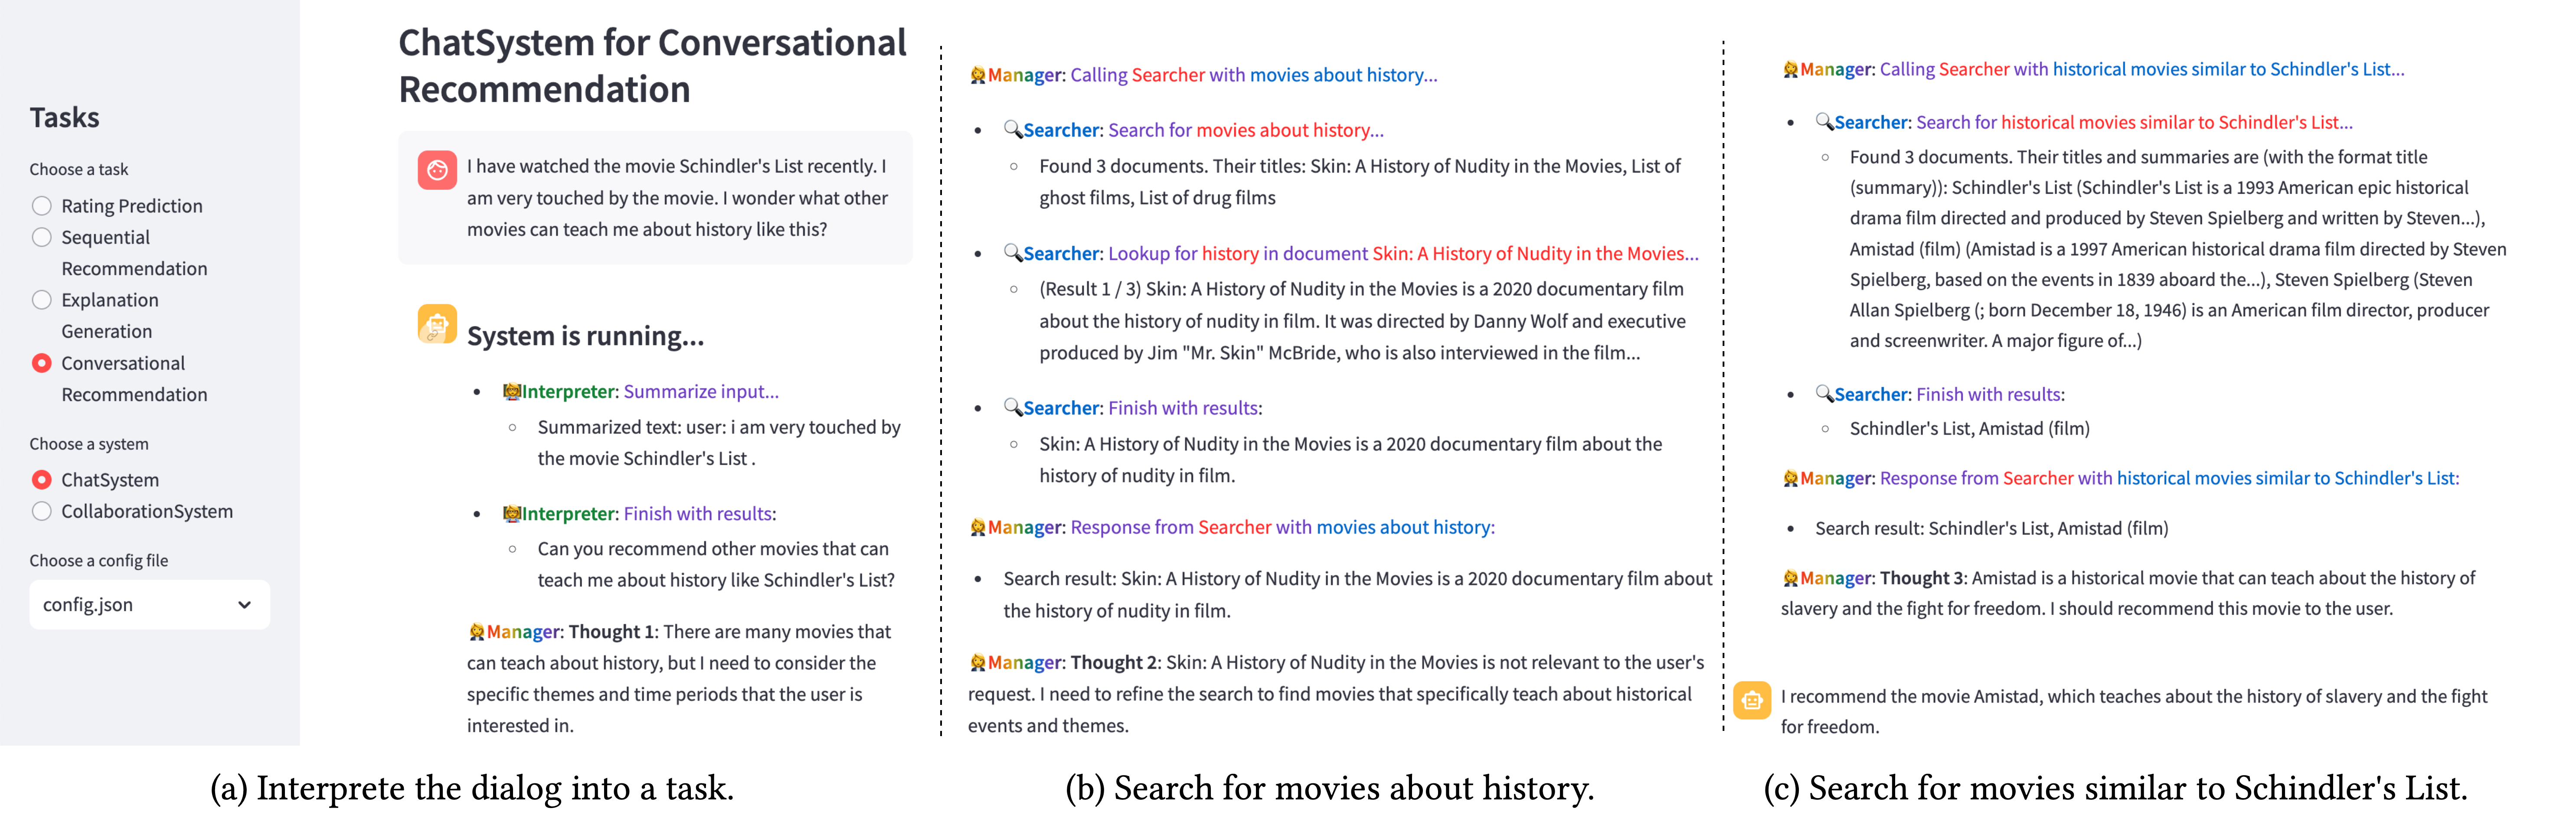
\includegraphics[trim={0 0 0 0}, clip, width=0.95\textwidth]{Figures/case_studypng.png}
\caption{The web interfaces of our MACRec, along with a case of how three agents collaboratively address a conversational recommendation task. The interface is composed by the leftmost configuration panel and the main interaction panel.}
\Description[The web interfaces of our MACRec.]{The web interfaces of our MACRec, along with a detailed case study demonstrating the collaborative efforts of three agents in addressing this task. The interface is composed by the leftmost configuration panel and the main interaction panel.}
\label{fig:case}
\end{figure*}
% A usage example of MACRec on a conversational recommendation task.  


Here, we present the applications of MACRec on four recommendation scenarios. Table~\ref{tab:application} summarizes the agents' selection for each scenario.

\begin{table}[h!]
    \centering
    \begin{tabular}{c|ccccc}
    \toprule
    Task & U.Analy. & I.Analy. & Reflector & Searcher & Interpreter \\
    \midrule
    RP & \usym{2611} & \usym{2611} & \usym{2610} \\
    SR & \usym{2611} & \usym{2610} & \usym{2611}\\
    EG & \usym{2611} & \usym{2611} & \usym{2610} & \usym{2611} \\
    CR & & & & \usym{2611} & \usym{2611} \\
    \bottomrule
    \end{tabular}
    \caption{The agents' selection for four applications supported by MACRec.\label{tab:application} \protect\usym{2611} means required and \protect\usym{2610} means optional.}
    \vspace{-3.0em}
\end{table}

\subsection{Rating Prediction (RP)}

% 介绍 Rating Prediction
Rating prediction task involves predicting the numerical rating a user might give to an item, such as a movie or a product, based on their preferences and historical interactions.

% 介绍 MAC
% 在评分预测任务中，每个用户会有不同的打分偏好。
In the rating prediction task, each user will have different rating preferences.
% User Analyst:
The \textsl{User Analyst} can provide a detailed analysis of the user's historical interactions and preferences.
% Item Analyst:
Meanwhile, the \textsl{Manager} also needs characteristic analysis of the target item, which can be provided by the \textsl{Item Analyst}.
% Manager:
% 在两种analyst的帮助下，Manager可以在打分前对于用户的打分倾向和物品的近期评分有具体的了解。
With the help of two types of \textsl{Analysts}, the \textsl{Manager} can know the user's tendency to rate and the item's recent ratings before giving a prediction.

% 我们为评分预测任务使用了Manager、Reflector 和 Analyst（可选的） 三种agent
% We used three agents, the \textsl{Manager}, the \textsl{Reflector}, and the \textsl{Analyst} (optional) for the rating prediction task.
% 我们选用 Reflector 对 Manager 在单轮中可能出现的错误进行识别和归因。
% We chose the \textsl{Reflector} to identify and attribute errors that may occur in a single round of the \textsl{Manager}.
% 同时，Analyst可以帮助更好的总结归纳用户与物品的特征，因此也被我们选取应用在评分预测任务中。
% Meanwhile, the \textsl{Analyst} can help better summarize user and item characteristics, so we also selected it to apply in the rating prediction task.
% For the rating prediction task, the task prompt contains the user's profile, historical interactions, and the target item that needs to be rated.

% yyq: 没有必要介绍prompt
% % 所有的item都会对应给出他们的Attributes，历史交互item还会额外给出用户对其的评分。
% All items will be given their attributes, and items in the user's historical interactions will also be given the user's ratings.
% The actor is asked to rate the target item with the format of \verb|Finish[rating]|, where \verb|rating| is a float number between 1 and 5.

\subsection{Sequential Recommendation (SR)}

% 介绍 Sequential Recommendation
Sequential recommendation systems analyze the sequence of items a user has interacted with to predict their next likely interest.

% 介绍 MAC
% 在序列推荐任务中，对于用户长短期兴趣的建模十分重要。
Modeling of user's long-term and short-term interests is important in sequential recommendation tasks.
Hence, the \textsl{User Analyst}'s role is self-evident.
% 与评分预测任务相比，(由于同时包含了用户的交互历史和候选物品列表)，序列推荐中相关的物品数量明显更多。
The number of relevant items in the sequence is significantly higher than the rating prediction task.
It is hard to ask the \textsl{Item Analyst} to analyze every item that appeared in either the history or the candidate set.
% Therefore, the role of the \textsl{Item Analyst} is comparatively limited compared to other scenarios.
% 而考虑到序列推荐任务的答案更为复杂，Reflector可以很好地帮助Manager发现答案格式上的问题。
Moreover, given that the answers to the sequential recommendation task are much more complex (i.e., a ranking order of the candidate set), the \textsl{Reflector} can help to avoid the \textsl{Manager} getting into formatting troubles.
% 并且单轮的行为分析中，可能遗漏对于用户长期行为的考虑，而对此的反思也是Reflector可以做到的。
A single round of behavioral analysis may omit consideration of long-term user behavior, and reflection on this is something the \textsl{Reflector} can do.

% 序列推荐任务的agents选取与评分预测基本一致。
% The agent selection for the sequence recommendation task is the same as the score prediction.
% 值得注意的是，由于序列推荐任务设定中给出的历史交互物品以及候选集物品的特征较多，由Analyst来负责具体的特征分析可以大大减轻Manager的上下文长度。
% It is worth noting that leveraging the \textsl{Analyst} to do characterization can greatly reduce the context length of the \textsl{Manager}.
% yyq: 没有必要介绍prompt
% For the sequential recommendation task, the task prompt contains the user's profile, historical interactions, and the candidate set that needs to be ranked.
% % 候选集中包含了用户真实的下一个交互item和若干个未交互的负样本。
% The candidate set contains the positive sample (the next item in the user's historical interactions) and several negative samples (items that the user has not interacted with).
% % 相关物品的Attributes也会如上给出。
% The attributes of the relevant items will also be given as above.
% The actor is asked to rank the candidate set with the format of \verb|Finish[rank]|, where \verb|rank| is a permutation of the item IDs of the candidate set.

\subsection{Explanation Generation (EG)}
% 介绍 Explanation Generation
This task involves generating understandable and relevant explanations for the recommendations provided to users.

% 介绍 MAC
The explanation generation task also requires a detailed analysis of both the user and the item.
In addition, more information about the item may also help the \textsl{Manager} understand the user's behavior towards it.
% 例如，用户可能对同一个导演的多部电影拥有相似的喜好，而这些信息不一定被数据集所包含。
For example, a user may have similar preferences for multiple movies by the same director.
The information about the director may not be contained in the dataset.
Retrieving these extra pieces of information is suitable for the \textsl{Searcher} to perform.

% 我们在解释生成任务上的设定与前两个任务基本一致。
% Our setup for the explanation generation task is similar to the first two tasks.
% 除了Reflector和Analyst以外，我们还选取了Searcher以满足解释生成对于具体物品（如电影）的进一步深入了解的需求。
% In addition to the \textsl{Reflector} and the \textsl{Analyst}, we selected the \textsl{Searcher} (optional) to satisfy the need for further insights into specific items (e.g., movies) for explanation generation.

\subsection{Conversational Recommendation (CR)}
% 介绍 Conversational Recommendation
Conversational recommender systems engage users in a dialogue to refine their preferences and deliver more accurate suggestions.

% 介绍 MAC
In conversational scenarios, the user's input text is not necessarily explicitly instructive.
Hence, the \textsl{Task Interpreter} can help translate the conversation history into a more concise and clear task prompt.
% 同时，用户的输入需求中可能包含Manager所不了解的物品信息。
In addition, the user's input requirements may contain information unknown to the \textsl{Manager}. % , e.g., a product that has not sold on the platform.
In this case, the \textsl{Searcher} can help the Manager understand what the user mentioned.

% Beyond the above applications, TODO
% 还可以支持其他的task，需要XXX可以支持
Beyond the abovementioned applications, our framework can support other scenarios by customizing the configurations.

% 对话场景下我们选取了Searcher和Task Interpreter作为对Manager的辅助。
% We selected the \textsl{Searcher} and the \textsl{Task Interpreter} for the dialog scenario as an aid to the \textsl{Manager}.
% 由于用户的输入文本并不一定具有明确的指示性，我们将完整的对话历史交由Task Interpreter进行转译后再交给Manager作为更直接的任务要求。
% Since the user's input text is not necessarily explicitly instructive, we use the \textsl{Task Interpreter} to translate the whole dialog history into a more direct task request for the \textsl{Manager}.
% 而LLM对用户提到的部分实体不一定有足够了解，因此我们还选取了Searcher作为额外知识的扩充。
% Considering that the LLM may not necessarily know enough about the entities mentioned by the users, we also selected the \textsl{Searcher} as an extension of additional knowledge.
% \subsection{Interactive Recommendation}
% % 介绍 Interactive Recommendation
% Interactive recommendation systems dynamically adjust their suggestions based on real-time feedback from the user. 

% % 介绍 MAC

% \subsection{Click-Through Rate Prediction}
% % 介绍 Click-Through Rate Prediction
% Click-Through Rate (CTR) prediction tasks focus on estimating the likelihood that a user will click on a given recommendation.

% % 介绍 MAC


% \subsection{Experimental Settings}
% \label{subsec: experimental settings}

% \subsubsection{\textbf{Datasets}}
% We conduct experiments on MovieLens-100k and Amazon Beauty, which are two widely used datasets for rating prediction and sequential recommendation.
% % 我们对两个数据集分别进行了leave-one-out的处理，得到了每个用户的历史行为序列，以及最后一条行为作为测试集。
% We process the two datasets with the leave-one-out strategy and obtain the historical interaction sequence of each user.
% The last interaction is used as the test set.

% % 对于序列推荐任务，我们为每条历史行为采样了9个负样本用于评测，并在加入prompt前统一打乱了顺序，
% For sequential recommendation, we sample 9 negative samples for each historical interaction for evaluation and shuffle the order before adding to the prompt.
% We only evaluate the performance of the positive sample in the test set, i.e. the rating to the target item given by the user is at least 4.

% % 两个数据集具体的划分如下：
% The specific division of the two datasets is as follows:
% \begin{itemize}
%     \item MovieLens-100k: 943 samples for test, 489 positive samples for sequential, 500 samples for each round training, 
%     \item Amazon Beauty: 1000 samples for test, 759 positive samples for sequential.
% \end{itemize}

% \subsubsection{\textbf{Implementation Details}} 

% % 对于API-based LLM的选取，我们默认使用了GPT-3.5 base。
% For API-based LLM, we select \verb|gpt-3.5-turbo| base as default.
% % 特别地，对于序列推荐任务，我们使用了GPT-3.5 JSON作为默认以尽可能保证actor和reflector输出格式的正确性。
% Especially, for the sequential recommendation, we use \verb|gpt-3.5-turbo-1106| and enable JSON mode as default to ensure the correctness of the output format of both agents.
% We set the temperature to 0 to ensure the stability of the output.

% For open-source LLM, we use \verb|vicuna-7b-v1.5-16k| as default. We set the temperature to 0.9 and the top-p to 1.0.

% For rating prediction, we use $0$ as the prediction of the answers with an invalid format.
% % 序列推荐任务中，我们仅选取了最近的20条历史行为作为输入，以保证模型输入的长度不会过长。
% For sequential recommendation, we only select the last 20 historical interactions as input to ensure that the length of the input is not too long.

% % 强调 single-agent multi-agent



% \subsection{Experimental Results}

% % 整体推荐性能表现
% The overall recommendation performance is shown in Table~\ref{tab:exp_rp} and Table~\ref{tab:exp_sr}. From the experimental results, we mainly have the following observations.


% % 1. 分析 Collaboration 效果
% Firstly, adding the reflector agent without training appears to decrease accuracy while increasing RMSE. This suggests that multi-agent collaboration in recommendation systems is a complex endeavor that requires meticulous design and targeted training to yield positive outcomes. The initial decline in performance may be attributed to the additional complexity and potential misalignment between the actor and reflector agents' objectives or methods of processing information.

% % 2. 分析 (multi-round) Train 效果
% Secondly, the experimental data indicates that multi-round training enhances the performance of the recommendation system. Specifically, the vicuna-7b reflector with a single round of training demonstrates an improvement over the untrained base model, as seen by the reduction in RMSE. This improvement is more pronounced after two training rounds, underscoring the benefits of iterative training processes. While further rounds of training were not conducted due to constraints of time and resources, there is an implication that additional training could lead to even greater enhancements in recommendation performance.

% % 3. 分析JSON mode的影响
% Last but not least, it is apparent from the GPT-3.5 JSON results that this model variant provides a significant performance boost. The JSON model variant achieves the highest accuracy and lowest RMSE on the MovieLens-100k dataset when functioning both as the actor and reflector. This improved performance could be due to the structured nature of the JSON format, which may facilitate better data interpretation and learning by the model. 





% \subsection{Case Study} % for demo paper

% actor's thought

% reflector's determination and reasoning